\documentclass[11pt]{article}

\usepackage[margin=0.75in]{geometry}
\usepackage[T1]{fontenc}
\usepackage{amsmath}
\usepackage{amssymb}
\usepackage{array}
\usepackage{booktabs}
\usepackage{longtable}
\usepackage{tabularx}
\usepackage{enumitem}
\usepackage{xcolor}
\usepackage{graphicx}
\usepackage{tikz}
\usetikzlibrary{arrows.meta,positioning,calc,fit,backgrounds}
\usepackage{listings}
\usepackage[hidelinks]{hyperref}

\emergencystretch=2em

\newcommand{\sig}[1]{\texttt{\detokenize{#1}}}
\newcommand{\file}[1]{\texttt{\detokenize{#1}}}
\newcommand{\param}[1]{\texttt{\detokenize{#1}}}
\newcommand{\statusword}[1]{\texttt{\detokenize{#1}}}
\newcommand{\bitrange}[1]{\texttt{[#1]}}
\newcommand{\logicone}{\texttt{1'b1}}
\newcommand{\logiczero}{\texttt{1'b0}}
\newcommand{\TODO}[1]{\textcolor{red}{\textbf{TODO:}~#1}}

\definecolor{cfblue}{RGB}{20,74,123}
\definecolor{cfgreen}{RGB}{21,105,72}
\definecolor{cfamber}{RGB}{146,91,17}
\definecolor{cfgray}{RGB}{245,247,250}
\definecolor{cfline}{RGB}{65,72,82}
\definecolor{cflight}{RGB}{252,253,255}

\lstdefinestyle{cfcode}{
  basicstyle=\ttfamily\small,
  keywordstyle=\color{cfblue}\bfseries,
  commentstyle=\color{cfgreen},
  stringstyle=\color{cfamber},
  numbers=left,
  numberstyle=\tiny\color{gray},
  stepnumber=1,
  numbersep=7pt,
  frame=single,
  rulecolor=\color{cfline},
  backgroundcolor=\color{cfgray},
  breaklines=true,
  columns=fullflexible,
  keepspaces=true,
  showstringspaces=false,
  tabsize=4
}
\lstset{style=cfcode}

\title{\textbf{CaelumFusion Flight Control System}\\
Source-Backed Architecture, Instrumentation, and Verification Report}
\author{Engineering Design Review Artifact}
\date{Source snapshot reviewed on 2026-07-06}

\begin{document}
\maketitle

\begin{abstract}
This report documents the CaelumFusion Flight Control System as implemented in
the local Vivado project tree \file{CaelumFusion_Flight_Control_System}.  The
document is written as a design-review and portfolio artifact: it describes what
the system does, how the major RTL blocks are organized, what the electrical and
protocol contracts are, and how correctness is established through simulation,
static implementation evidence, Digilent WaveForms instrumentation, CSV export,
and MATLAB analysis.  Claims are intentionally separated into implemented RTL
facts, documented build evidence, and pending hardware-capture work.  The
dominant verification objective is not merely to display telemetry, but to
preserve a traceable evidence chain from physical pins and bus transactions to
decoded CSV files, MATLAB plots, and reportable engineering conclusions.
\end{abstract}

\noindent\textbf{Keywords:}
FPGA instrumentation; Basys 3; Artix-7; Digilent WaveForms; MATLAB
telemetry analysis; I2C; SPI; VGA HUD; clock-domain crossing; fixed-point
flight visualization.

\tableofcontents
\newpage

\section*{Nomenclature and Notation}
\addcontentsline{toc}{section}{Nomenclature and Notation}

\begin{longtable}{@{}p{0.18\textwidth}p{0.73\textwidth}@{}}
\toprule
Symbol or term & Meaning used in this document \\
\midrule
\endfirsthead
\toprule
Symbol or term & Meaning used in this document \\
\midrule
\endhead
\sig{SYS} & The primary 100 MHz FPGA logic domain driven from the Basys 3 oscillator. \\
\sig{PIX} & The VGA pixel-rendering domain, nominally 25 MHz for 640 by 480 timing. \\
\sig{CDC} & Clock-domain crossing.  The report uses this term only for explicit synchronizer, snapshot, toggle, or reset-domain interfaces. \\
\sig{snapshot} & A committed sensor record containing timestamp, sequence number, validity, status, payload, and age metadata. \\
\sig{status} & Eight-bit semantic health field defined in \file{telemetry_defs_vh.vh}.  \sig{ST_OK} is the only normal valid status. \\
\sig{age_ms} & Millisecond age of a committed snapshot relative to the SYS-domain timebase. \\
\sig{Qm.n} & Fixed-point format with $m$ integer/sign bits and $n$ fractional bits.  The attitude CORDIC uses Q4.12 radians and Q1.15 trigonometric outputs. \\
\sig{mdeg} & Millidegrees.  The HUD uses this integer unit for roll and heading display fields. \\
\sig{ACK} & I2C acknowledge bit; in the report's pass/fail wording, an address ``ACK'' means the target pulled SDA low during the acknowledge bit. \\
\sig{WF-001}--\sig{WF-003} & Planned WaveForms evidence captures defined in \file{captures/README.md}. \\
\bottomrule
\end{longtable}

\section{Introduction and Purpose}
\label{sec:purpose}

The CaelumFusion Flight Control System is a Basys 3 / Artix-7 FPGA design that
acquires sensor telemetry, derives flight-state observables, renders a VGA
flight visualization, and exposes enough debug structure to validate the
hardware in a repeatable bench workflow.  The active top-level RTL is
\file{caelumfusion_top_vga.v}.  The current default build favors a
resource-safe Basys 3 configuration: the shared-I2C sensor path, CMPS2 heading
publication, PMON/HYGRO/GYRO support, and MAG1 bench source are compiled by
default, while the ADXL362 SPI accelerometer path and optional high-cost VGA
diagnostic pages remain parameter-selectable.

The purpose of this report is fourfold:

\begin{enumerate}[leftmargin=*]
  \item define the implemented architecture and its clock, reset, dataflow, and
        control-flow contracts;
  \item define the physical probe and CSV evidence workflow required to validate
        the FPGA-to-sensor interfaces using Digilent WaveForms;
  \item describe how exported WaveForms data is converted into MATLAB plots and
        derived engineering measurements; and
  \item document what is currently proven, what remains pending, and what risks
        should be retired before the design is treated as flight-evidence grade.
\end{enumerate}

The report uses the following evidence boundary.  RTL and XDC facts are
grounded in files under \file{CaelumFusion_Flight_Control_System.srcs}.  WaveForms
and MATLAB workflow facts are grounded in the local documentation and capture
manifest under \file{docs} and \file{captures}.  Timing/resource status is
reported as the documented baseline from the release checklist, not as a fresh
implementation run performed by this report.

\section{Motivation, Problem Statement, and Scope}
\label{sec:motivation-scope}

The engineering problem is not only to connect sensors to an FPGA.  The harder
problem is to preserve a reviewable chain of meaning from a physical bus edge
to a displayed or plotted engineering conclusion.  A flight-control display can
be visually convincing while still being wrong if the physical interface is
miswired, if a stale snapshot is plotted as fresh, if an optional build path is
assumed to be active when it is compiled out, or if a clock-domain crossing
samples a multi-bit value without a stable transfer contract.  CaelumFusion is
therefore organized around explicit ownership boundaries: sensor engines own
bus transactions, snapshot registers own semantic publication, the extension
hub owns freshness and plausibility status, the visualization CDC owns
SYS-to-PIX transfer, and the pixel renderer owns only frame-domain rendering.

The scope of this final draft is the implemented Basys 3 VGA-oriented flight
control and observability build.  It includes the default shared-I2C sensor
configuration, the optional ADXL362 SPI build path, the extension hub, the
apogee authority telemetry model, VGA/HUD rendering, WaveForms capture
contracts, and MATLAB analysis workflow.  It does not claim completed physical
sensor validation until the corresponding \sig{WF-*} captures have been
archived.  Unsupported or pending evidence is marked with \TODO{...} instead of
being described as a completed result.

\subsection{System Objectives}
\label{subsec:objectives}

The system objectives are:

\begin{enumerate}[leftmargin=*]
  \item acquire pressure, acceleration, magnetometer, power, environmental,
        and auxiliary extension data through explicitly owned sensor interfaces;
  \item publish committed snapshots with timestamps, sequence numbers, status,
        validity, payload, and age metadata;
  \item compute derived altitude, vertical speed, roll, heading, freshness, and
        apogee-authority observables in deterministic SYS-domain logic;
  \item move visualization state across the SYS-to-PIX boundary using a stable
        snapshot/toggle CDC contract rather than asynchronous bitwise sampling;
  \item render a VGA HUD and diagnostic views whose visible state can be tied
        back to packed telemetry fields; and
  \item validate physical bus behavior using WaveForms CSV evidence and
        reproducible MATLAB plots.
\end{enumerate}

\begin{table}[htbp]
\centering
\caption{Primary source files used as design evidence.}
\label{tab:sources}
\small
\begin{tabularx}{\textwidth}{@{}p{0.35\textwidth}X@{}}
\toprule
Source & Evidence used in this report \\
\midrule
\file{caelumfusion_top_vga.v} &
Top-level parameters, physical ports, runtime switch controls, sensor-suite
integration, render-control integration, and current idle-high UART assignment. \\
\file{rocket_i2c_suite_top.v} &
Sensor acquisition layers, shared-I2C policy, ADXL362 SPI availability,
cadence policy, observability counters, and derived-state publication bank. \\
\file{sensor_extension_hub.v} &
Extension freshness limits, MAG redundancy checks, status mapping, fault flags,
and diagnostic fault-injection behavior. \\
\file{flight_viz_bundle_cdc.v} &
SYS-to-PIX snapshot transfer contract, toggle-event synchronizer, and wide-bus
CDC assumptions. \\
\file{flight_viz_suite_top.v} and \file{flight_visualizer_pix.v} &
Visualization bundle handoff, frame-domain rendering, history buffers, page
multiplexing, and VGA timing integration. \\
\file{flight_viz_bundle_defs.vh} and \file{telemetry_defs_vh.vh} &
Packed visualization bit fields, source identifiers, status identifiers, and
extension flag definitions. \\
\file{Basys-3-Master.xdc} &
Clock definition, top-level pin locations, I/O standards, pullups, and CDC false
path constraints. \\
\file{CaelumFusion_WaveForms_to_MATLAB_Workflow.md} &
Bench probe plan, WaveForms decoder settings, CSV schema, MATLAB processing
stages, and anomaly checks. \\
\file{captures/README.md} &
Capture-manifest contract and planned reportable captures WF-001 through
WF-003. \\
\bottomrule
\end{tabularx}
\end{table}

\section{System Requirements}
\label{sec:requirements}

The system requirements in Table~\ref{tab:reqs} combine implemented RTL
contracts with bench-evidence requirements.  The distinction matters: a signal
can be correctly implemented in RTL and still not yet be validated as a
physical bench interface until the corresponding WaveForms capture exists in
the manifest.

\begin{longtable}{@{}p{0.13\textwidth}p{0.21\textwidth}p{0.46\textwidth}p{0.13\textwidth}@{}}
\caption{System requirements and verification approach.}
\label{tab:reqs}\\
\toprule
ID & Requirement & Acceptance criterion & Evidence mode \\
\midrule
\endfirsthead
\toprule
ID & Requirement & Acceptance criterion & Evidence mode \\
\midrule
\endhead
REQ-SYS-001 & Deterministic SYS-domain acquisition &
All sensor jobs are driven from a fixed-rate SYS-domain timebase and fixed
priority arbitration.  Jobs do not directly drive the shared I2C pins; one
shared engine owns bus drive behavior. & RTL review, simulation \\
REQ-SYS-002 & Stable physical clock &
The Basys 3 \sig{clk} input is constrained to a 10.000 ns period, giving
$f_{\mathrm{SYS}}=100~\mathrm{MHz}$. & XDC, timing report \\
REQ-SYS-003 & VGA video timing &
The pixel pipeline renders 640 by 480 active pixels with nominal 25 MHz pixel
timing and 800 by 525 total timing counts. & RTL, display bench \\
REQ-SENS-001 & BMP585 I2C presence &
With only the BMP585 attached to JA, the I2C decode shall show a 7-bit address
\sig{0x47} transaction with ACK and no SDA contention. & WF-001 capture \\
REQ-SENS-002 & CMPS2 I2C presence &
With BMP585 plus CMPS2 and SW9 enabled, the I2C decode shall show a 7-bit
address \sig{0x30} transaction with ACK while preserving BMP585 ACK behavior. &
WF-002 capture \\
REQ-SENS-003 & ADXL362 SPI identity &
Only after a bitstream with \param{USE_ADXL362_SPI_ACC=1}, the SPI decode shall
show a valid ADXL362 identity read with \sig{PARTID=0xF2}. & WF-003 capture \\
REQ-OBS-001 & Traceable telemetry evidence &
Each reportable bench run shall archive raw CSV, decoded CSV, plots, bitstream
identity, switch state, and attached Pmods in the capture manifest. & Manifest \\
REQ-CDC-001 & Explicit CDC boundary &
The wide visualization bundle shall cross from SYS to PIX as a stable snapshot
with a synchronized event toggle; individual data bits are not treated as
independent asynchronous signals. & RTL, XDC \\
REQ-VIZ-001 & Frame-stable visualization &
HUD-visible state shall be committed in the pixel domain through the
visualization pipeline, preserving active-video gating and deterministic page
selection. & Simulation, display bench \\
REQ-ANA-001 & Reproducible MATLAB analysis &
CSV imports shall be schema-checked, cleaned without silent data loss, converted
to physical/protocol units, plotted, and compared against expected contracts. &
MATLAB script, plots \\
\bottomrule
\end{longtable}

\begin{table}[htbp]
\centering
\caption{Requirements-to-deliverables traceability.}
\label{tab:traceability}
\small
\begin{tabularx}{\textwidth}{@{}p{0.15\textwidth}p{0.31\textwidth}p{0.44\textwidth}@{}}
\toprule
Requirement & Implemented or planned deliverable & Review evidence \\
\midrule
REQ-SYS-001, REQ-SYS-002 & \file{rocket_i2c_suite_top}, \file{timebase_us}, top-level \param{SYS_CLK_HZ} & RTL source review, XDC clock constraint, scheduler/counter simulation. \\
REQ-SENS-001, REQ-SENS-002 & Shared-I2C physical capture plan & \sig{WF-001} and \sig{WF-002} raw CSV, decoded CSV, MATLAB address/ACK plots. \\
REQ-SENS-003 & ADXL362 diagnostic bitstream and SPI capture plan & \sig{WF-003} raw CSV, decoded SPI bytes, \sig{PARTID=0xF2} check. \\
REQ-CDC-001 & \file{flight_viz_bundle_cdc} and XDC false-path intent & RTL inspection, CDC-focused simulation, no bitwise asynchronous bundle use. \\
REQ-VIZ-001 & \file{flight_visualizer_pix}, \file{flight_vga_page_mux_pix}, and HUD diagrams & Pixel testbench, frame screenshots, active-video gating checks. \\
REQ-OBS-001, REQ-ANA-001 & \file{captures/README.md} and \file{tools/matlab/analyze_waveforms_capture.m} & Manifest rows, MATLAB generated plots, anomaly table, archived bitstream/switch state. \\
\bottomrule
\end{tabularx}
\end{table}

\section{Hardware Platform}
\label{sec:platform}

\subsection{FPGA Board}

The documented target is the Digilent Basys 3 development board containing a
Xilinx Artix-7 \sig{xc7a35tcpg236-3}.  The top-level clock is the board 100 MHz
oscillator on package pin W5, constrained as shown in
Listing~\ref{lst:xdc-clock}.  The reset input \sig{rst} is mapped to package pin
U18.  All listed user I/O is constrained as \sig{LVCMOS33}.

\begin{lstlisting}[language=Verilog,caption={Clock contract from the Basys 3 XDC.},label={lst:xdc-clock}]
set_property PACKAGE_PIN W5 [get_ports clk]
set_property IOSTANDARD LVCMOS33 [get_ports clk]
create_clock -add -name sys_clk_pin -period 10.00 -waveform {0 5} [get_ports clk]
\end{lstlisting}

\subsection{Sensor and Debug Connectors}

The design uses the Basys 3 Pmod banks as both sensor interfaces and Digilent
Discovery probe targets.  The critical rule for bench capture is to probe the
FPGA-side signal at the Pmod header or immediately adjacent signal pad, not at a
distant flying lead after the sensor module.  This makes the CSV evidence
represent what the FPGA actually drove or sampled.

\begin{longtable}{@{}p{0.12\textwidth}p{0.14\textwidth}p{0.14\textwidth}p{0.18\textwidth}p{0.33\textwidth}@{}}
\caption{Physical signal and probe-location contract.}
\label{tab:pins}\\
\toprule
Discovery DIO & Report name & FPGA signal & Basys 3 package pin & Probe location and purpose \\
\midrule
\endfirsthead
\toprule
Discovery DIO & Report name & FPGA signal & Basys 3 package pin & Probe location and purpose \\
\midrule
\endhead
DIO0 & \sig{i2c_scl} & \sig{scl} & J2 & JA SCL at FPGA-side Pmod header; I2C clock decode and bus timing. \\
DIO1 & \sig{i2c_sda} & \sig{sda} & G2 & JA SDA at FPGA-side Pmod header; I2C data, ACK/NACK, bus idle, and contention. \\
DIO2 & \sig{acl2_cs_n} & \sig{adxl362_cs_n} & A14 & JB ACL2 chip select; active-low SPI frame boundary. \\
DIO3 & \sig{acl2_mosi} & \sig{adxl362_mosi} & A16 & JB MOSI; FPGA-to-ADXL362 command/address/data stream. \\
DIO4 & \sig{acl2_miso} & \sig{adxl362_miso} & B15 & JB MISO; ADXL362-to-FPGA response stream. \\
DIO5 & \sig{acl2_sclk} & \sig{adxl362_sclk} & B16 & JB SCLK; SPI timing reference. \\
DIO6 & \sig{acl2_int1} & \sig{adxl362_int1} & A17 & JB INT1; data-ready interrupt when enabled by policy. \\
DIO7 & \sig{acl2_int2} & \sig{adxl362_int2} & A15 & JB INT2; optional interrupt policy input. \\
DIO8--DIO11 & \sig{ls1_s[3:0]} & \sig{ls1_s_raw[3:0]} & K17, M18, N17, P18 & JC GPIO level evidence; synchronized into SYS domain. \\
DIO12 & \sig{pir_motion} & \sig{pir_motion_raw} & L17 & JC PIR motion evidence; synchronized into SYS domain. \\
DIO13 & \sig{dpot_cs_n} & \sig{dpot_cs_n} & M19 & JC digital potentiometer CS. \\
DIO14 & \sig{dpot_mosi} & \sig{dpot_mosi} & P17 & JC digital potentiometer MOSI. \\
DIO15 & \sig{dpot_sclk} & \sig{dpot_sclk} & R18 & JC digital potentiometer SCLK. \\
\bottomrule
\end{longtable}

\subsection{Runtime Switches and Buttons}

The top-level design exposes runtime controls through synchronized switches and
buttons.  These controls are important in hardware validation because the CSV
capture is only meaningful when the manifest records the switch state that
selected the active sensor path.

\begin{table}[htbp]
\centering
\caption{Selected runtime controls relevant to bench validation.}
\label{tab:switches}
\small
\begin{tabularx}{\textwidth}{@{}p{0.20\textwidth}p{0.17\textwidth}X@{}}
\toprule
Top-level signal & XDC package pin & Validation role \\
\midrule
\sig{sw_lis3dh_i2c_acc_raw} & W13 & Enables the LIS3DH I2C accelerometer path when compiled. \\
\sig{sw_adxl362_spi_acc_raw} & V2 & Runtime gate for the ADXL362 SPI path, but only meaningful when the bitstream compiled that path. \\
\sig{sw_cmps2_mmc3416_mag_raw} & T3 & Runtime gate for the CMPS2/MMC3416 magnetometer job on the shared I2C bus. \\
\sig{sw_pmon1_pwr_raw} & T2 & Runtime gate for PMON1/ADM1191 shared-I2C publication. \\
\sig{sw_mag1_bench_raw} & W17 & Selects MAG1 bench-source publication when the bench source is compiled. \\
\sig{sw_compass_page_raw} & W15 & Legacy compass-page hold control; page must also be compiled into the build. \\
\sig{sw_history_freeze_raw} & V15 & Freezes history update behavior for visual inspection. \\
\sig{btn_page_raw}, \sig{btn_prev_raw}, \sig{btn_direct_compass_raw} & T18, U17, T17 & Debounced page-control inputs feeding the render-control subsystem. \\
\bottomrule
\end{tabularx}
\end{table}

\section{Architecture Overview}
\label{sec:architecture}

At a high level, CaelumFusion is organized into a SYS-domain acquisition and
control side, a CDC boundary, and a PIX-domain visualization side.  The SYS side
owns sensors, synchronized controls, telemetry status, extension-hub policy,
derived-state publication, and history write intent.  The PIX side owns VGA
timing, HUD page multiplexing, active-video gating, and the final RGB/HSYNC/VSYNC
outputs.

Figure~\ref{fig:architecture} summarizes the principal dataflow.  The diagram
uses a left-to-right convention: physical inputs enter on the left, SYS-domain
semantic processing occurs in the middle-left, the CDC boundary is explicit, and
PIX-domain rendering exits to the right.

\begin{figure}[htbp]
\centering
\resizebox{\textwidth}{!}{%
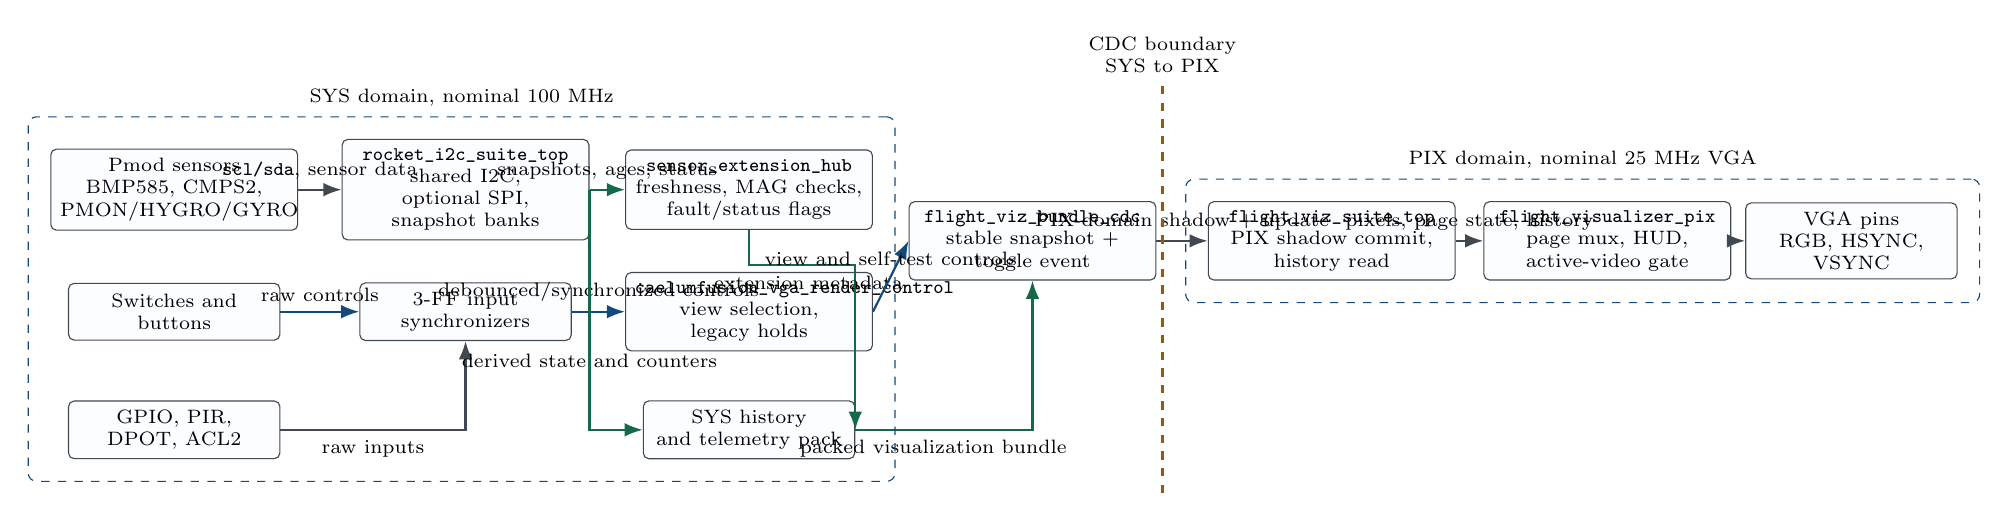
\begin{tikzpicture}[
    >=Latex,
    font=\scriptsize,
    block/.style={draw=cfline, fill=cflight, rounded corners=2pt, align=center,
                  minimum height=0.88cm, text width=2.9cm},
    smallblock/.style={draw=cfline, fill=cflight, rounded corners=2pt, align=center,
                  minimum height=0.72cm, text width=2.45cm},
    domainbox/.style={draw=cfblue, dashed, rounded corners=3pt, inner sep=0.28cm},
    cdc/.style={draw=cfamber, very thick, dashed},
    wire/.style={->, thick, draw=cfline},
    ctrlwire/.style={->, thick, draw=cfblue},
    statuswire/.style={->, thick, draw=cfgreen}
]

\node[block] (pmods) at (0,2.2) {Pmod sensors\\BMP585, CMPS2,\\PMON/HYGRO/GYRO};
\node[smallblock] (switches) at (0,0.65) {Switches and\\buttons};
\node[smallblock] (gpio) at (0,-0.85) {GPIO, PIR,\\DPOT, ACL2};

\node[block] (suite) at (3.7,2.2) {\file{rocket_i2c_suite_top}\\shared I2C, optional SPI,\\snapshot banks};
\node[smallblock] (syncs) at (3.7,0.65) {3-FF input\\synchronizers};
\node[block] (hub) at (7.3,2.2) {\file{sensor_extension_hub}\\freshness, MAG checks,\\fault/status flags};
\node[block] (control) at (7.3,0.65) {\file{caelumfusion_vga_render_control}\\view selection, legacy holds};
\node[smallblock] (history) at (7.3,-0.85) {SYS history\\and telemetry pack};

\node[block] (cdc) at (10.9,1.55) {\file{flight_viz_bundle_cdc}\\stable snapshot +\\toggle event};
\node[block] (pixsuite) at (14.7,1.55) {\file{flight_viz_suite_top}\\PIX shadow commit,\\history read};
\node[block] (renderer) at (18.2,1.55) {\file{flight_visualizer_pix}\\page mux, HUD,\\active-video gate};
\node[smallblock] (vga) at (21.3,1.55) {VGA pins\\RGB, HSYNC, VSYNC};

\draw[wire] (pmods.east) -- node[above]{\sig{scl/sda}, sensor data} (suite.west);
\draw[wire] (gpio.east) -| node[pos=0.25,below]{raw inputs} (syncs.south);
\draw[ctrlwire] (switches.east) -- node[above]{raw controls} (syncs.west);
\draw[ctrlwire] (syncs.east) -- node[above]{debounced/synchronized controls} (control.west);
\draw[statuswire] (suite.east) -- node[above]{snapshots, ages, status} (hub.west);
\draw[statuswire] (suite.east) |- node[pos=0.32,below]{derived state and counters} (history.west);
\draw[statuswire] (hub.south) -- ++(0,-0.45) -| node[pos=0.28,below]{extension metadata} (history.east);
\draw[ctrlwire] (control.east) -- node[above]{view and self-test controls} (cdc.west);
\draw[statuswire] (history.east) -| node[pos=0.22,below]{packed visualization bundle} (cdc.south);
\draw[wire] (cdc.east) -- node[above]{PIX-domain shadow + update} (pixsuite.west);
\draw[wire] (pixsuite.east) -- node[above]{pixels, page state, history} (renderer.west);
\draw[wire] (renderer.east) -- (vga.west);

\draw[cdc] (12.55,-1.65) -- (12.55,3.55) node[above,align=center]{CDC boundary\\SYS to PIX};
\node[domainbox, fit=(pmods)(switches)(gpio)(suite)(syncs)(hub)(control)(history), label={[align=center]above:SYS domain, nominal 100 MHz}] {};
\node[domainbox, fit=(pixsuite)(renderer)(vga), label={[align=center]above:PIX domain, nominal 25 MHz VGA}] {};

\end{tikzpicture}%
}
\caption{Source-backed block architecture.  Sensor and control semantics are
formed in the SYS clock domain; the visualization bundle crosses one explicit
CDC boundary before pixel-domain VGA rendering.}
\label{fig:architecture}
\end{figure}

\section{Clock and Reset Organization}
\label{sec:clock-reset}

\subsection{SYS Clock}

The primary clock contract is
\begin{equation}
    f_{\mathrm{SYS}} = 100~\mathrm{MHz}, \qquad
    T_{\mathrm{SYS}} = \frac{1}{f_{\mathrm{SYS}}}=10~\mathrm{ns}.
    \label{eq:sys-clock}
\end{equation}
The top-level parameter \param{SYS_CLK_HZ} is set to \sig{100_000_000}.  This
constant drives the microsecond timebase used by the sensor suite and is also
the reference for low-rate scheduling and telemetry ages.

\subsection{VGA Pixel Timing}

The active VGA format is 640 by 480.  The timing parameters are:
\begin{equation}
\begin{aligned}
H_{\mathrm{tot}} &= H_{\mathrm{active}} + H_{\mathrm{fp}} + H_{\mathrm{sync}} + H_{\mathrm{bp}}
                 = 640 + 16 + 96 + 48 = 800,\\
V_{\mathrm{tot}} &= V_{\mathrm{active}} + V_{\mathrm{fp}} + V_{\mathrm{sync}} + V_{\mathrm{bp}}
                 = 480 + 10 + 2 + 33 = 525.
\end{aligned}
\label{eq:vga-totals}
\end{equation}
With a nominal 25 MHz pixel clock, the nominal frame rate is therefore
\begin{equation}
    f_{\mathrm{frame}} =
    \frac{25\,000\,000}{800\cdot525}
    \approx 59.52~\mathrm{Hz}.
    \label{eq:vga-frame}
\end{equation}
The design uses a dedicated VGA timing generator in the pixel domain.  The
rendering contract is that RGB is meaningful only inside active video and that
page-specific renderers are selected through deterministic page mux logic.

\subsection{Reset Policy}

Reset is intentionally local to each major synchronous domain.  SYS-domain
logic resets sensor state, telemetry registers, synchronized controls, and
history writers.  PIX-domain logic resets timing, page commit state, and the
shadow visualization bundle.  CDC modules reset their source-side and
destination-side state independently.  This is the correct reset topology for a
design in which semantic telemetry publication and visible frame commit are
separate events.

\section{Dataflow and Control Flow}
\label{sec:dataflow}

\subsection{Sensor Dataflow}

The acquisition pipeline implemented by \file{rocket_i2c_suite_top.v} is
structured as five layers: timebase, cadence intent, per-sensor jobs, shared bus
engine ownership, and committed snapshot publication.  This organization is
important because it prevents leaf job modules from becoming implicit bus
masters.  All shared-I2C bus behavior is serialized through the shared engine.

The committed snapshot contract is:
\begin{equation}
    \mathrm{snapshot} =
    \{t_{\mu s},\ \mathrm{seq},\ \mathrm{source\_id},\ \mathrm{status},\
      \mathrm{valid},\ \mathrm{payload},\ \mathrm{age}_{ms}\}.
    \label{eq:snapshot}
\end{equation}
Derived-state publication is computed from committed snapshots, not from
partially updated bus transaction state.  This gives the visualizer and
extension hub a stable semantic input contract.

\subsection{Control Flow}

Runtime control inputs first cross through synchronizers and debouncers before
affecting view selection, self-test gating, sensor publication gates, or history
freeze behavior.  The render-control block accepts next/previous/direct-view
pulses and legacy hold controls, then produces a resolved effective view.  The
current implemented view identifiers are summarized in
Table~\ref{tab:viewids}.

\begin{table}[htbp]
\centering
\caption{Render-control view identifiers.}
\label{tab:viewids}
\small
\begin{tabularx}{\textwidth}{@{}p{0.14\textwidth}p{0.24\textwidth}X@{}}
\toprule
ID & Symbol & Contract \\
\midrule
\sig{3'd0} & \sig{VIEW_FLIGHT_HUD} & Normal telemetry HUD. \\
\sig{3'd1} & \sig{VIEW_COMPASS_TRUTH} & Full-screen compass/magnetometer truth page when the page is compiled into the build. \\
\sig{3'd2} & \sig{VIEW_SELFTEST_HUD} & Normal HUD with self-test stimulus enabled. \\
\sig{3'd3} & \sig{VIEW_SENSOR_DIAG} & HUD renderer diagnostics page when selected. \\
Other & invalid & Rejected by the render-control legal-view function and reflected through invalid-view status. \\
\bottomrule
\end{tabularx}
\end{table}

\begin{figure}[htbp]
\centering
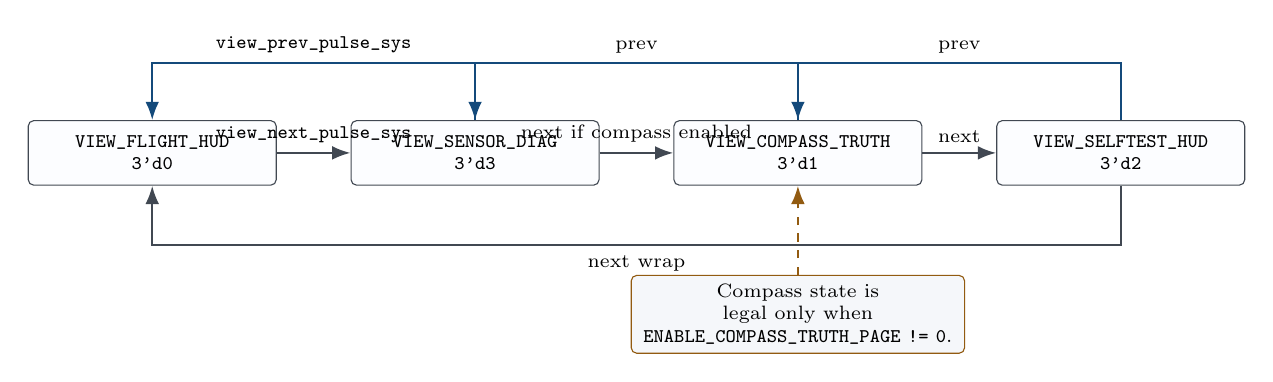
\begin{tikzpicture}[
  >=Latex,
  font=\scriptsize,
  state/.style={draw=cfline, fill=cflight, rounded corners=2pt, align=center,
                minimum width=3.15cm, minimum height=0.82cm},
  note/.style={draw=cfamber, fill=cfgray, rounded corners=2pt, align=center,
               text width=4.0cm, minimum height=0.72cm},
  next/.style={->, thick, draw=cfline},
  prev/.style={->, thick, draw=cfblue},
  gate/.style={->, thick, dashed, draw=cfamber}
]
\node[state] (hud) at (0,0) {\sig{VIEW_FLIGHT_HUD}\\\sig{3'd0}};
\node[state] (diag) at (4.1,0) {\sig{VIEW_SENSOR_DIAG}\\\sig{3'd3}};
\node[state] (compass) at (8.2,0) {\sig{VIEW_COMPASS_TRUTH}\\\sig{3'd1}};
\node[state] (self) at (12.3,0) {\sig{VIEW_SELFTEST_HUD}\\\sig{3'd2}};
\node[note] (off) at (8.2,-2.05) {Compass state is legal only when \param{ENABLE_COMPASS_TRUTH_PAGE != 0}.};

\draw[next] (hud.east) -- node[above]{\sig{view_next_pulse_sys}} (diag.west);
\draw[next] (diag.east) -- node[above]{next if compass enabled} (compass.west);
\draw[next] (compass.east) -- node[above]{next} (self.west);
\draw[next] (self.south) -- ++(0,-0.75) -| node[pos=0.25,below]{next wrap} (hud.south);

\draw[prev] (diag.north) -- ++(0,0.72) -| node[pos=0.25,above]{\sig{view_prev_pulse_sys}} (hud.north);
\draw[prev] (compass.north) -- ++(0,0.72) -| node[pos=0.25,above]{prev} (diag.north);
\draw[prev] (self.north) -- ++(0,0.72) -| node[pos=0.25,above]{prev} (compass.north);
\draw[gate] (off.north) -- (compass.south);
\end{tikzpicture}
\caption{Implemented view-selection state machine in \file{caelumfusion_vga_render_control.v}.  Direct requests have priority over next/previous pulses; illegal direct IDs do not move \sig{view_sel_sys} and latch \sig{cfg_invalid_view_sys}.}
\label{fig:view-fsm}
\end{figure}

\section{Module Hierarchy}
\label{sec:hierarchy}

Table~\ref{tab:hierarchy} lists the report-relevant hierarchy rather than every
leaf renderer.  The intent is to show ownership boundaries: sensor acquisition,
extension policy, CDC, and pixel rendering are not interchangeable concerns.

\begin{longtable}{@{}p{0.29\textwidth}p{0.22\textwidth}p{0.41\textwidth}@{}}
\caption{Functional module hierarchy and ownership.}
\label{tab:hierarchy}\\
\toprule
Module & Clock/domain & Engineering role \\
\midrule
\endfirsthead
\toprule
Module & Clock/domain & Engineering role \\
\midrule
\endhead
\file{caelumfusion_top_vga} & SYS and PIX integration & Top-level physical ports, parameters, synchronized controls, sensor-suite instantiation, extension hub, render control, VGA output path. \\
\file{rocket_i2c_suite_top} & SYS & Canonical sensor acquisition suite; shared-I2C engine, optional ADXL362 SPI engine, committed snapshots, derived-state outputs, counters. \\
\file{sensor_extension_hub} & SYS & Extension metadata aggregation, freshness checks, MAG redundancy checks, fault/status mapping, diagnostic fault injection. \\
\file{mag1_bench_snapshot_source} & SYS & Synthetic or bench MAG1 snapshot publication for redundancy validation when compiled and enabled. \\
\file{caelumfusion_vga_render_control} & SYS with PIX output integration & Resolves view requests, legacy page holds, self-test view state, invalid-view status, and visualizer controls. \\
\file{flight_viz_bundle_cdc} & SYS to PIX & Transfers the packed visualization bundle by stable source hold register plus synchronized toggle event. \\
\file{flight_viz_suite_top} & SYS/PIX boundary and PIX & Bridges visualization data into pixel-domain rendering and manages history/page integration. \\
\file{flight_visualizer_pix} & PIX & Owns VGA timing, page muxing, HUD rendering, text/plot composition, active-video gating, and final RGB/HSYNC/VSYNC. \\
\file{vga_timing_640x480_60} & PIX & Generates counters, active-video mask, sync pulses, and frame timing events. \\
\bottomrule
\end{longtable}

\section{Interface and Signal Contracts}
\label{sec:contracts}

\subsection{Sensor Protocol Contracts}

The primary sensor interfaces are summarized in Table~\ref{tab:protocols}.  The
default top-level parameters compile the shared-I2C path and leave the ADXL362
SPI path available only by parameter override.

\begin{table}[htbp]
\centering
\caption{Sensor protocol contracts.}
\label{tab:protocols}
\small
\begin{tabularx}{\textwidth}{@{}p{0.16\textwidth}p{0.16\textwidth}p{0.16\textwidth}X@{}}
\toprule
Interface & Nominal rate & Compile/runtime gate & Contract \\
\midrule
BMP585 / BMP58x I2C & 100 kHz bus; 50 Hz job cadence & Shared-I2C suite & Reportable hardware evidence shall show 7-bit address \sig{0x47} ACK. \\
CMPS2 / MMC3416 I2C & 100 kHz bus; 10 Hz job cadence & \param{USE_CMPS2_MMC3416_MAG=1}, SW9 gate & Reportable hardware evidence shall show 7-bit address \sig{0x30} ACK when enabled. \\
PMON1 / ADM1191 I2C & 100 kHz bus; 10 Hz job cadence & \param{USE_PMON1_PWR=1}, SW10 gate, address \sig{0x38} & Power telemetry appears as a shared-I2C snapshot when enabled. \\
HYGRO environment I2C & 100 kHz bus; 1 Hz job cadence & \param{USE_HYGRO_ENV=1} & Environment snapshot uses extension freshness/status policy. \\
GYRO I2C & 100 kHz bus; 10 Hz job cadence & \param{USE_GYRO_I2C=1} & Gyro snapshot participates in raw/derived telemetry where compiled. \\
ADXL362 / Pmod ACL2 SPI & 1 MHz SPI & \param{USE_ADXL362_SPI_ACC=0} by default; enable in diagnostic bitstream & Mode-0, active-low CS, MSB-first, 8-bit words; identity proof is \sig{PARTID=0xF2}. \\
\bottomrule
\end{tabularx}
\end{table}

The current top-level default parameters relevant to the sensor stack are shown
in Listing~\ref{lst:top-params}.  This listing explains why the ADXL362 SPI
capture is not expected to show active traffic under the default bitstream.

\begin{lstlisting}[language=Verilog,caption={Default top-level sensor parameters.},label={lst:top-params}]
parameter [15:0] BUILD_ID    = 16'd4,
parameter integer ADXL_IRQ_POLICY = 1,
parameter integer USE_LIS3DH_I2C_ACC    = 1,
parameter integer USE_ADXL362_SPI_ACC   = 0,
parameter integer USE_CMPS2_MMC3416_MAG = 1,
parameter integer USE_PMON1_PWR         = 1,
parameter [6:0]   PMON1_ADDR7           = 7'h38,
parameter integer USE_HYGRO_ENV         = 1,
parameter integer USE_GYRO_I2C          = 1,
parameter integer USE_LIS2MDL_MAG1      = 0,
parameter integer USE_BLACKBOX_LOG      = 0,
parameter integer USE_MAG1_BENCH_SOURCE = 1
\end{lstlisting}

\subsection{Telemetry Source and Status Identifiers}

The telemetry contract uses explicit source and status enumerations.  Selected
values are shown in Table~\ref{tab:source-status}.  MATLAB analysis should never
treat a nonzero status field as benign unless the corresponding plot is
explicitly a fault plot.

\begin{table}[htbp]
\centering
\caption{Selected telemetry source and status identifiers.}
\label{tab:source-status}
\small
\begin{tabularx}{\textwidth}{@{}p{0.16\textwidth}p{0.19\textwidth}X@{}}
\toprule
Class & Identifier & Meaning \\
\midrule
Source & \sig{SRC_BMP58X_RAW = 8'h01} & BMP585/BMP58x pressure snapshot source. \\
Source & \sig{SRC_LIS3DH_RAW = 8'h02} & LIS3DH auxiliary acceleration source. \\
Source & \sig{SRC_LIS2MDL_RAW = 8'h03} & Legacy redundant magnetometer source identifier. \\
Source & \sig{SRC_ALTITUDE_DERIVED = 8'h10} & Derived altitude publication. \\
Source & \sig{SRC_HEADING_DERIVED = 8'h13} & Derived heading publication. \\
Source & \sig{SRC_MAG_REDUNDANCY_EVID = 8'h30} & MAG redundancy/extension evidence. \\
Status & \sig{ST_OK = 8'h00} & Valid and accepted. \\
Status & \sig{ST_I2C_NACK = 8'h03} & I2C target did not acknowledge. \\
Status & \sig{ST_SENSOR_ID_MISMATCH = 8'h05} & Device identity check failed. \\
Status & \sig{ST_PLAUSIBILITY_REJECT = 8'h09} & Physical or cross-sensor plausibility check rejected data. \\
Status & \sig{ST_STALE_REJECT = 8'h0A} & Data was present but too old for the freshness contract. \\
Status & \sig{ST_MISSING_INPUT = 8'h0B} & A required redundant or derived input is missing. \\
Status & \sig{ST_CDC_MISSED_UPDATE = 8'h0D} & CDC publication accounting detected a missed update. \\
\bottomrule
\end{tabularx}
\end{table}

\subsection{Extension Fault and Presence Bit Fields}

The extension hub produces a compact diagnostic record.  Presence bits indicate
what subsystems are represented; fault bits explain why an extension status is
not \statusword{ST_OK}.  The important analysis rule is to plot both the status
word and the decomposed fault bits.  A single aggregate status is insufficient
to diagnose whether a capture failed because of staleness, plausibility, raw
sensor status, or intentionally injected diagnostic fault state.

\begin{longtable}{@{}p{0.20\textwidth}p{0.16\textwidth}p{0.55\textwidth}@{}}
\caption{Extension flag bit map.}
\label{tab:extension-flags}\\
\toprule
Field & Bit & Meaning \\
\midrule
\endfirsthead
\toprule
Field & Bit & Meaning \\
\midrule
\endhead
\sig{ext_present_flags} & 0 & Primary magnetometer represented. \\
\sig{ext_present_flags} & 1 & Redundant MAG1 represented. \\
\sig{ext_present_flags} & 2 & Range/height source represented. \\
\sig{ext_present_flags} & 3 & Air-data source represented. \\
\sig{ext_present_flags} & 4 & Environment source represented. \\
\sig{ext_present_flags} & 7 & Blackbox/log source represented. \\
\sig{ext_present_flags} & 8 & Diagnostic source represented. \\
\sig{ext_fault_flags} & 0 & MAG pair missing. \\
\sig{ext_fault_flags} & 1 & MAG pair disagreement. \\
\sig{ext_fault_flags} & 2--3 & Primary or redundant MAG norm out of range. \\
\sig{ext_fault_flags} & 4 & MAG norm mismatch. \\
\sig{ext_fault_flags} & 5--9 & Range, air, environment, sun, or flow stale. \\
\sig{ext_fault_flags} & 10 & Raw status error propagated from an input bank. \\
\sig{ext_fault_flags} & 11 & Blackbox/log drop. \\
\sig{ext_fault_flags} & 12 & Diagnostic fault injection active. \\
\bottomrule
\end{longtable}

\subsection{Visualization Bundle Bit Fields}

The packed visualization bundle width is \sig{VIZ_BUNDLE_W=1152}.  Selected
high-value fields are listed in Table~\ref{tab:viz-bits}.  These bit positions
are important for debug because a bitfield packing mistake can produce a
visually plausible HUD with semantically wrong units.

\begin{longtable}{@{}p{0.26\textwidth}p{0.18\textwidth}p{0.47\textwidth}@{}}
\caption{Selected visualization bundle bit-field map.}
\label{tab:viz-bits}\\
\toprule
Field & Bits & Contract \\
\midrule
\endfirsthead
\toprule
Field & Bits & Contract \\
\midrule
\endhead
\sig{VIZ_EXT_VALID_BIT} & 1151 & Extension summary valid flag. \\
\sig{VIZ_EXT_STATUS} & 1150:1143 & Extension status word. \\
\sig{VIZ_EXT_PRESENT} & 1142:1127 & Extension presence flags. \\
\sig{VIZ_EXT_FAULT} & 1126:1111 & Extension fault flags. \\
\sig{VIZ_EXT_MAG_DELTA_L1} & 1110:1095 & MAG pair L1 disagreement metric. \\
\sig{VIZ_EXT_MAG_NORM0} & 1094:1079 & Primary MAG norm. \\
\sig{VIZ_EXT_MAG_NORM1} & 1078:1063 & Redundant MAG norm. \\
\sig{VIZ_EXT_RNG_HEIGHT_CM} & 1062:1047 & Range/height in centimeters. \\
\sig{VIZ_EXT_AIR_DP_PA} & 1046:1031 & Differential pressure in pascals. \\
\sig{VIZ_EXT_AIR_SPEED_CMS} & 1030:1015 & Airspeed in centimeters per second. \\
\sig{VIZ_EXT_ENV_TEMP_CDEG} & 1014:999 & Environment temperature in centi-degrees Celsius. \\
\sig{VIZ_EXT_ENV_RH_CENTI} & 998:983 & Relative humidity in centi-percent. \\
\sig{VIZ_DER_ALT_CM} & 244:213 & Derived altitude in centimeters. \\
\sig{VIZ_DER_VSPD_CMS} & 212:181 & Derived vertical speed in centimeters per second. \\
\sig{VIZ_DER_ROLL_MDEG} & 180:149 & Derived roll in millidegrees. \\
\sig{VIZ_DER_HEAD_MDEG} & 148:117 & Derived heading in millidegrees. \\
\sig{VIZ_DER_I2C_NACK} & 116:101 & I2C NACK count. \\
\sig{VIZ_DER_I2C_TIMEOUT} & 100:85 & I2C timeout count. \\
\sig{VIZ_DER_TXN_RATE} & 84:69 & Shared-bus transaction rate. \\
\sig{VIZ_DER_BUILD_ID} & 36:5 & Build identifier. \\
\sig{VIZ_DER_SCHEMA_WORD} & 4:1 & Visualization schema word. \\
\bottomrule
\end{longtable}

\section{Timing and CDC Strategy}
\label{sec:timing-cdc}

\subsection{Protocol Timing}

The shared I2C engine is instantiated with a nominal bus rate of
\begin{equation}
    f_{\mathrm{I2C}} = 100~\mathrm{kHz}.
    \label{eq:i2c}
\end{equation}
For WaveForms validation, each SCL period should therefore be approximately
\begin{equation}
    T_{\mathrm{SCL}} = \frac{1}{100\,000}=10~\mu\mathrm{s}.
    \label{eq:i2c-period}
\end{equation}
The ADXL362 SPI engine, when compiled, is instantiated with
\begin{equation}
    f_{\mathrm{SPI}} = 1~\mathrm{MHz}, \qquad
    T_{\mathrm{SCLK}} = 1~\mu\mathrm{s}.
    \label{eq:spi-period}
\end{equation}

\begin{table}[htbp]
\centering
\caption{Bench timing settings derived from the implemented protocol rates.}
\label{tab:bench-timing}
\small
\begin{tabularx}{\textwidth}{@{}p{0.16\textwidth}p{0.18\textwidth}p{0.17\textwidth}X@{}}
\toprule
Capture type & Suggested sample rate & Trigger & Capture duration \\
\midrule
I2C address/ACK validation & 10 to 25 MS/s & START condition or SDA falling while SCL high & 20 to 100 ms; enough for multiple scheduler epochs and ACK observations. \\
ADXL362 SPI identity validation & 25 to 100 MS/s & Falling edge of \sig{acl2_cs_n} & 2 to 20 ms; enough to include command, address, dummy, and response bytes. \\
GPIO/PIR/DPOT debug & 1 to 10 MS/s for slow GPIO; 25 MS/s for DPOT SPI-like edges & Edge on signal of interest & Event dependent; record the manifest trigger explicitly. \\
Analog signal-integrity spot check & Analog Scope 1 to 10 MS/s & Edge or normal acquisition & Short captures around transitions; verify logic-high, logic-low, rise/fall, and overshoot. \\
\bottomrule
\end{tabularx}
\end{table}

\subsection{CDC Strategy}

The most important CDC path is the visualization bundle transfer from SYS to
PIX.  It is not a bitwise synchronizer.  Instead, the source domain latches a
wide semantic bundle into a hold register, toggles a one-bit event marker, and
the destination domain synchronizes the event marker before sampling the held
bundle.  This is appropriate because visualization publications are low-rate
relative to the pixel clock and the held bundle remains stable until the next
publish event.

\begin{lstlisting}[language=Verilog,caption={Implemented visualization snapshot CDC pattern.},label={lst:cdc}]
always @(posedge src_clk) begin
    if (src_rst) begin
        src_bundle_hold <= {BUNDLE_W{1'b0}};
        src_toggle      <= 1'b0;
    end else if (src_publish_pulse) begin
        src_bundle_hold <= src_bundle;
        src_toggle      <= ~src_toggle;
    end
end

(* ASYNC_REG = "TRUE", SHREG_EXTRACT = "NO" *) reg [2:0] dst_toggle_sync_ff;

always @(posedge dst_clk) begin
    if (dst_rst) begin
        dst_toggle_sync_ff <= 3'b000;
    end else begin
        dst_toggle_sync_ff[0] <= src_toggle;
        dst_toggle_sync_ff[1] <= dst_toggle_sync_ff[0];
        dst_toggle_sync_ff[2] <= dst_toggle_sync_ff[1];
    end
end

assign dst_toggle_changed = (dst_toggle_sync_ff[2] ^ dst_toggle_sync_ff[1]);

always @(posedge dst_clk) begin
    if (dst_rst) begin
        dst_bundle_shadow <= {BUNDLE_W{1'b0}};
        dst_update_pulse  <= 1'b0;
    end else begin
        dst_update_pulse <= 1'b0;
        if (dst_toggle_changed) begin
            dst_bundle_shadow <= src_bundle_hold;
            dst_update_pulse  <= 1'b1;
        end
    end
end
\end{lstlisting}

The XDC marks the CDC intent with false paths for the snapshot hold-to-shadow
path and the toggle synchronizer input.  Additional false paths are defined for
asynchronous buttons, switches, ADXL interrupt inputs, history freeze controls,
and the diagnostic page selector.

\begin{figure}[htbp]
\centering
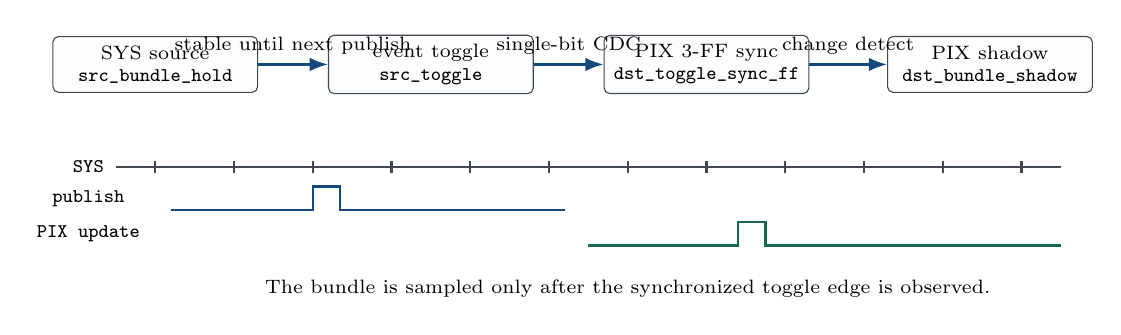
\begin{tikzpicture}[
  >=Latex,
  font=\scriptsize,
  sigline/.style={thick, draw=cfline},
  edge/.style={->, thick, draw=cfblue},
  box/.style={draw=cfline, fill=cflight, rounded corners=2pt, align=center,
              minimum width=2.6cm, minimum height=0.65cm}
]
\node[box] (src) at (0,1.2) {SYS source\\\sig{src_bundle_hold}};
\node[box] (tog) at (3.5,1.2) {event toggle\\\sig{src_toggle}};
\node[box] (sync) at (7.0,1.2) {PIX 3-FF sync\\\sig{dst_toggle_sync_ff}};
\node[box] (dst) at (10.6,1.2) {PIX shadow\\\sig{dst_bundle_shadow}};

\draw[edge] (src.east) -- node[above]{stable until next publish} (tog.west);
\draw[edge] (tog.east) -- node[above]{single-bit CDC} (sync.west);
\draw[edge] (sync.east) -- node[above]{change detect} (dst.west);

\draw[sigline] (-0.5,-0.1) -- (11.5,-0.1);
\foreach \x in {0,1,2,3,4,5,6,7,8,9,10,11}
  \draw[sigline] (\x,-0.18) -- (\x,-0.02);
\node[align=right] at (-0.85,-0.1) {\sig{SYS}};
\draw[sigline, cfblue] (0.2,-0.65) -- (2.0,-0.65) -- (2.0,-0.35) -- (2.35,-0.35) -- (2.35,-0.65) -- (5.2,-0.65);
\node[align=right] at (-0.85,-0.5) {\sig{publish}};
\draw[sigline, cfgreen] (5.5,-1.1) -- (7.4,-1.1) -- (7.4,-0.8) -- (7.75,-0.8) -- (7.75,-1.1) -- (11.5,-1.1);
\node[align=right] at (-0.85,-0.95) {\sig{PIX update}};
\node[align=center] at (6.0,-1.65) {The bundle is sampled only after the synchronized toggle edge is observed.};
\end{tikzpicture}
\caption{Conceptual timing of the implemented visualization CDC.  The wide data bundle is held stable in SYS; only the event toggle is synchronized bitwise into PIX.}
\label{fig:cdc-timing}
\end{figure}

\section{Mathematical Model and Theory of Operation}
\label{sec:theory}

\subsection{Attitude Extraction from Sensor Vectors}
\label{subsec:attitude-theory}

The implemented attitude math is contained in \file{flight_attitude_math_sys.v}.
The module does not attempt a full inertial navigation solution.  It computes
two display-oriented observables from sequence-qualified vector snapshots:
\begin{equation}
    \phi = \operatorname{atan2}(a_y,a_z),
    \qquad
    \psi = \operatorname{wrap}_{[0,2\pi)}\left(\operatorname{atan2}(m_y,m_x)\right),
    \label{eq:attitude}
\end{equation}
where $\phi$ is roll and $\psi$ is heading.  The implemented accelerometer
payload contract is \sig{{AX[15:0], AY[15:0], AZ[15:0]}} for the ADXL362/ACL2
path.  The implemented magnetometer contract for the current MMC3416/CMPS2 path
is \sig{{MZ[15:0], MY[15:0], MX[15:0]}} because
\param{MAG_PAYLOAD_ZYX=1}.  The implemented wire bindings use AY and AZ for
roll, and MY and MX for heading; optional compile-time sign corrections are
applied before the CORDIC launch.

The hardware strategy is intentionally serialized.  One shared
\file{cordic_atan2_q12} services roll first and then heading.  This saves logic
relative to duplicating the CORDIC and is adequate because the sensor snapshot
rates are slow compared with the 100 MHz SYS clock.  A new vector is accepted
only when its source sequence changes, the source status is \sig{ST_OK}, and the
chosen two-axis vector is nonzero.  The commit pulses
\sig{roll_update} and \sig{head_update} are asserted after the corresponding
registers and sequence references have been updated, which gives downstream
snapshot logic a coherent one-cycle publication event.

\subsection{Fixed-Point Angle Representation}
\label{subsec:fixed-point}

The CORDIC angle is represented as Q4.12 radians:
\begin{equation}
    \theta_{\mathrm{rad}} \approx \frac{\theta_{\mathrm{Q12}}}{2^{12}}.
    \label{eq:q12-angle}
\end{equation}
The implemented constants are \param{PI_Q12=12868} and
\param{TWO_PI_Q12=25736}.  The display path converts Q4.12 radians to
millidegrees using a shift-add approximation:
\begin{equation}
    \theta_{\mathrm{mdeg}} \approx
    14\cdot\theta_{\mathrm{Q12}}
    =
    \left(\theta_{\mathrm{Q12}}\ll 4\right)
    -
    \left(\theta_{\mathrm{Q12}}\ll 1\right).
    \label{eq:q12-mdeg}
\end{equation}
The exact conversion factor is
\begin{equation}
    \frac{180\,000}{\pi\,2^{12}} \approx 13.988.
    \label{eq:mdeg-exact}
\end{equation}
Thus the implemented multiplier of 14 millidegrees per Q4.12 count is a small
integer approximation chosen to avoid a DSP in an always-live SYS path.  The
trigonometric outputs use signed Q1.15 values for display vectors:
\begin{equation}
    s_{\mathrm{Q15}} \approx \operatorname{round}(32767\sin\theta),
    \qquad
    c_{\mathrm{Q15}} \approx \operatorname{round}(32767\cos\theta).
    \label{eq:q15}
\end{equation}

\subsection{Apogee Authority Model}
\label{subsec:apogee-theory}

The apogee authority logic is implemented in
\file{apogee_authority_policy_sys.v}.  It is a deterministic policy model for
display, telemetry, and gated actuator demand; it is not yet a calibrated
aerodynamic model.  Its no-brake prediction starts from the textbook ballistic
estimate:
\begin{equation}
    h_{\mathrm{apogee,no}} = h + \frac{v_+^2}{2g},
    \qquad
    v_+ = \max(v,0),
    \label{eq:ballistic}
\end{equation}
with $h$ in centimeters, $v$ in centimeters per second, and
$g\approx981~\mathrm{cm/s^2}$.  The RTL approximation is:
\begin{equation}
    \frac{v_+^2}{2g} \approx
    \frac{33\,v_+^2}{2^{16}},
    \label{eq:coast-approx}
\end{equation}
which corresponds to an effective divisor of approximately 1985, close to
$2g=1962$.  The full-brake prediction uses half the computed coast height:
\begin{equation}
    h_{\mathrm{apogee,full}} =
    h + \frac{1}{2}\left(\frac{33\,v_+^2}{2^{16}}\right).
    \label{eq:full-brake}
\end{equation}
The uncertainty band combines a fixed base term with a linear age penalty:
\begin{equation}
    u = \min\left(U_{\max}, U_0 + 20\,\mathrm{cm/ms}\cdot
        \mathrm{der\_bmp\_age\_ms}\right),
    \label{eq:uncertainty}
\end{equation}
where the current RTL parameters are $U_0=1500~\mathrm{cm}$,
$U_{\max}=50000~\mathrm{cm}$, and
$h_{\mathrm{target}}=304800~\mathrm{cm}$, corresponding to 10,000 ft.

The command output is quantized into five levels:
\begin{equation}
    \sig{auth\_brake\_cmd\_u8}\in\{0,64,128,192,255\},
    \qquad
    \sig{auth\_servo\_us}\in\{1000,1250,1500,1750,2000\}.
    \label{eq:servo-levels}
\end{equation}
The raw brake command remains observable even when actuation is denied, but the
servo pulse retracts to \sig{1000 us} unless
\sig{safety_runtime_ok}, \sig{safety_allows_actuation},
\sig{policy_runtime_enable}, and \sig{software_armed} allow actuation.  This
separation is an important safety and observability invariant: policy demand
and physical actuator permission are not conflated.

\subsection{Coordinate-System and Rendering Assumptions}
\label{subsec:coordinates}

The pixel renderer uses VGA coordinates with origin at the upper-left active
pixel:
\begin{equation}
    x\in[0,639],\qquad y\in[0,479],
    \label{eq:vga-coords}
\end{equation}
where increasing $x$ moves right and increasing $y$ moves down.  The renderer
therefore maps increasing altitude or authority margin to smaller $y$ values.
For example, the implemented altitude tape and chart functions follow the
general form
\begin{equation}
    y(h)=y_1-\frac{\operatorname{clip}(h,0,h_{\max})(y_1-y_0)}{h_{\max}},
    \label{eq:y-map}
\end{equation}
with saturation rather than wraparound.  Signed quantities such as vertical
speed are mapped around a centerline:
\begin{equation}
    y(v)=y_c-\frac{\operatorname{clip}(v,-v_{\max},v_{\max})(y_1-y_0)}{2v_{\max}}.
    \label{eq:vspd-map}
\end{equation}
This coordinate convention is why plot validation must compare both the numeric
bundle fields and the direction of visible movement on the screen.

\subsection{Model Limitations}
\label{subsec:model-limitations}

The implemented models are deliberately bounded.  The roll estimate ignores
linear acceleration and treats the selected accelerometer axes as a gravity
vector.  The heading estimate is a two-axis magnetometer heading and does not
perform tilt compensation.  The apogee authority model uses a coarse ballistic
energy estimate and a half-energy full-brake proxy rather than a calibrated drag
model.  These limitations are acceptable for the current objective because the
system is being validated first as a deterministic telemetry, visualization, and
instrumentation platform.  Flight-accuracy claims require future calibration
data, higher-fidelity dynamics, and measured bench/field validation.

\section{Telemetry and Observability}
\label{sec:observability}

The design deliberately exposes observability beyond the plotted physical value.
For a reportable capture, the useful evidence is not only ``heading changed'' or
``altitude plotted.''  The report must also show whether the input was valid,
fresh, correctly identified, not stale, and not rejected by a cross-sensor
contract.

\subsection{Freshness and Fault Contracts}

The extension hub uses explicit freshness limits.  MAG inputs have
\param{MAG_FRESH_MAX_MS=300}; generic extension inputs have
\param{GENERIC_FRESH_MAX_MS=500}.  The basic freshness predicate is
\begin{equation}
    \mathrm{fresh}(x) =
    \mathrm{valid}(x)\ \land\
    \left(\mathrm{status}(x)=\mathrm{ST\_OK}\right)\ \land\
    \left(\mathrm{age}_{ms}(x)\le A_{\max}(x)\right).
    \label{eq:freshness}
\end{equation}
The MAG disagreement metric uses an L1 bound,
\begin{equation}
    \Delta_{\mathrm{MAG,L1}} =
    |m_{0x}-m_{1x}| + |m_{0y}-m_{1y}| + |m_{0z}-m_{1z}|,
    \qquad
    \Delta_{\mathrm{MAG,L1}} \le 2048.
    \label{eq:mag-l1}
\end{equation}
An observed violation maps into extension fault flags and then into a status
word for plausibility rejection, stale data, configuration error, or missing
input.  MATLAB plots should therefore include both the metric and its
binary/fault interpretation.

\subsection{CSV Evidence Schema}

The preferred CSV schema is one file per capture stage: a raw WaveForms digital
export, a decoded protocol CSV, and an optional normalized MATLAB-ready table.
The normalized table should preserve the fields in Table~\ref{tab:csv-schema}.

\begin{longtable}{@{}p{0.20\textwidth}p{0.17\textwidth}p{0.54\textwidth}@{}}
\caption{Recommended normalized CSV schema for MATLAB analysis.}
\label{tab:csv-schema}\\
\toprule
Column & Units/type & Description \\
\midrule
\endfirsthead
\toprule
Column & Units/type & Description \\
\midrule
\endhead
\sig{capture_id} & string & Manifest identifier, for example \sig{WF-001}. \\
\sig{time_s} & seconds & Reconstructed timebase relative to capture start. \\
\sig{sample_index} & count & Digital sample index from WaveForms export when available. \\
\sig{i2c_scl}, \sig{i2c_sda} & logic 0/1 & Thresholded I2C bus waveforms. \\
\sig{acl2_cs_n}, \sig{acl2_mosi}, \sig{acl2_miso}, \sig{acl2_sclk} & logic 0/1 & Thresholded SPI waveforms when the ADXL path is captured. \\
\sig{decoder} & categorical & Decoder source such as \sig{I2C}, \sig{SPI}, or \sig{UART}. \\
\sig{event_type} & categorical & START, STOP, ADDRESS, ACK, NACK, DATA, CS\_FALL, CS\_RISE, byte, or derived event. \\
\sig{addr7} & hex/integer & I2C 7-bit address for address events. \\
\sig{rw} & bit & I2C read/write bit. \\
\sig{ack} & bit/logical & ACK state, where true means acknowledged by the target. \\
\sig{mosi_byte}, \sig{miso_byte} & uint8 & SPI decoded bytes. \\
\sig{uart_byte} & uint8 & UART decoded byte if a future bitstream enables UART telemetry. \\
\sig{signal_name} & string & Name of the measured signal for long-form tables. \\
\sig{value_raw} & numeric/string & Raw decoded value before unit conversion. \\
\sig{value_si} & numeric & Converted engineering value where applicable. \\
\sig{status} & integer/string & Protocol or telemetry status field. \\
\sig{notes} & string & Human-readable anomaly or setup note. \\
\bottomrule
\end{longtable}

\section{Visualization and HUD Rendering}
\label{sec:visualization}

The visualization path should be understood as an engineering instrument rather
than a decorative display.  It renders the current telemetry contract, not
necessarily the live raw bus transaction.  The rendering pipeline therefore
separates raw acquisition from committed snapshots, extension policy, CDC
arrival, frame-domain commit, and final pixel composition.

The pixel-domain renderer owns:
\begin{itemize}[leftmargin=*]
  \item VGA timing counters and active-video gating;
  \item page selection and deterministic page multiplexing;
  \item text, plot, status, and HUD compositing;
  \item history readout for strip-chart style telemetry; and
  \item final \sig{vga_rgb[11:0]}, \sig{vga_hsync}, and \sig{vga_vsync} outputs.
\end{itemize}

Because the packed visualization bundle contains both physical values and
metadata, display validation should compare the rendered behavior against
decoded fields, not only against subjective visual appearance.  For example, a
heading plot with a nonzero \statusword{ST_STALE_REJECT} status is not valid
heading evidence; it is evidence that the stale-data visual path is working.

\begin{figure}[htbp]
\centering
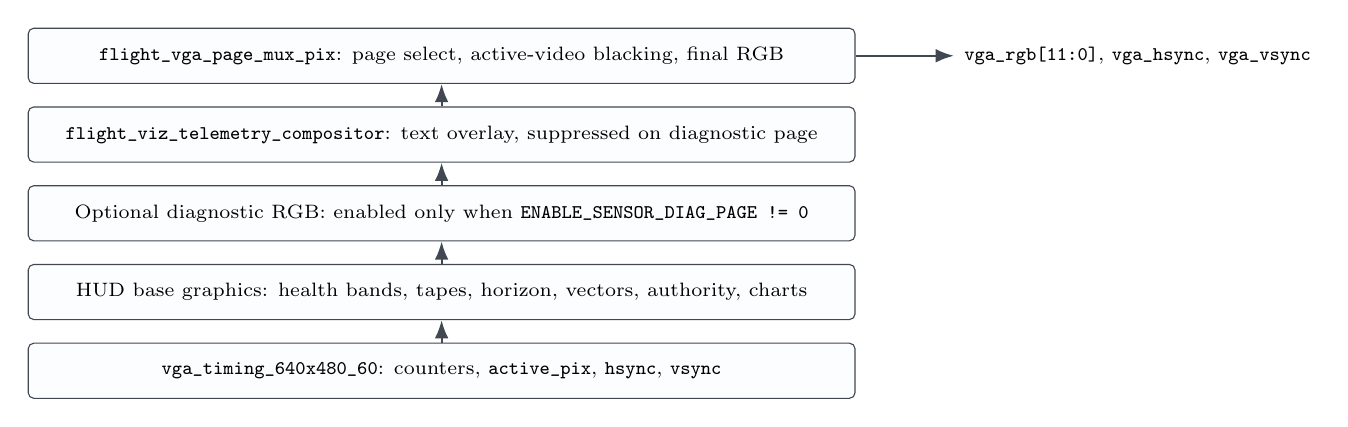
\begin{tikzpicture}[
  >=Latex,
  font=\scriptsize,
  layer/.style={draw=cfline, fill=cflight, rounded corners=2pt, align=center,
                minimum width=10.5cm, minimum height=0.7cm},
  wire/.style={->, thick, draw=cfline}
]
\node[layer] (timing) at (0,0) {\file{vga_timing_640x480_60}: counters, \sig{active_pix}, \sig{hsync}, \sig{vsync}};
\node[layer] (base) at (0,1.0) {HUD base graphics: health bands, tapes, horizon, vectors, authority, charts};
\node[layer] (diag) at (0,2.0) {Optional diagnostic RGB: enabled only when \param{ENABLE_SENSOR_DIAG_PAGE != 0}};
\node[layer] (text) at (0,3.0) {\file{flight_viz_telemetry_compositor}: text overlay, suppressed on diagnostic page};
\node[layer] (mux) at (0,4.0) {\file{flight_vga_page_mux_pix}: page select, active-video blacking, final RGB};
\draw[wire] (timing.north) -- (base.south);
\draw[wire] (base.north) -- (diag.south);
\draw[wire] (diag.north) -- (text.south);
\draw[wire] (text.north) -- (mux.south);
\draw[wire] (mux.east) -- ++(1.25,0) node[right]{\sig{vga_rgb[11:0]}, \sig{vga_hsync}, \sig{vga_vsync}};
\end{tikzpicture}
\caption{Pixel-domain compositor stack.  The implemented final mux blanks RGB outside active video and applies telemetry text only to the primary HUD page, matching \file{flight_vga_page_mux_pix.v}.}
\label{fig:compositor-stack}
\end{figure}

\begin{figure}[htbp]
\centering
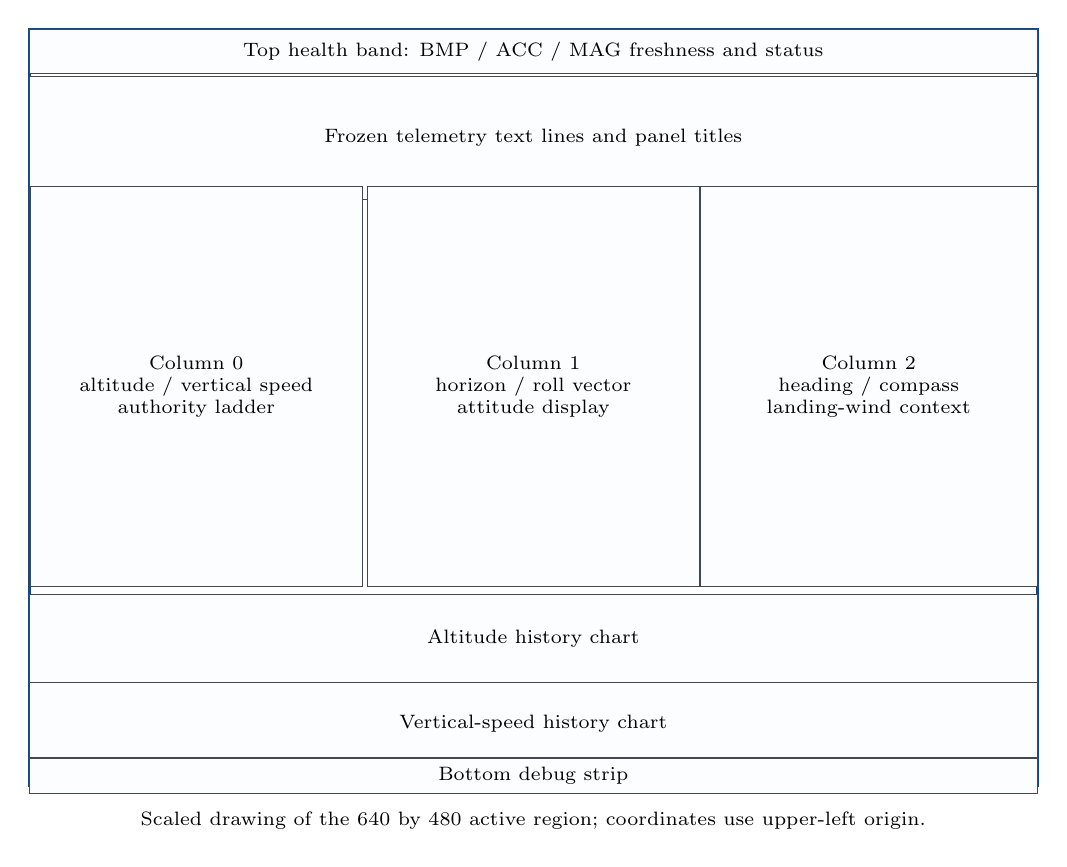
\begin{tikzpicture}[
  font=\scriptsize,
  region/.style={draw=cfline, fill=cflight, align=center},
  major/.style={draw=cfblue, very thick}
]
\draw[major] (0,0) rectangle (12.8,9.6);
\node[region, minimum width=12.8cm, minimum height=0.56cm] at (6.4,9.32) {Top health band: BMP / ACC / MAG freshness and status};
\node[region, minimum width=12.8cm, minimum height=1.56cm] at (6.4,8.22) {Frozen telemetry text lines and panel titles};
\node[region, minimum width=4.22cm, minimum height=5.08cm] at (2.12,5.06) {Column 0\\altitude / vertical speed\\authority ladder};
\node[region, minimum width=4.22cm, minimum height=5.08cm] at (6.4,5.06) {Column 1\\horizon / roll vector\\attitude display};
\node[region, minimum width=4.28cm, minimum height=5.08cm] at (10.66,5.06) {Column 2\\heading / compass\\landing-wind context};
\node[region, minimum width=12.8cm, minimum height=1.12cm] at (6.4,1.86) {Altitude history chart};
\node[region, minimum width=12.8cm, minimum height=1.04cm] at (6.4,0.78) {Vertical-speed history chart};
\node[region, minimum width=12.8cm, minimum height=0.24cm] at (6.4,0.12) {Bottom debug strip};
\node[align=center] at (6.4,-0.45) {Scaled drawing of the 640 by 480 active region; coordinates use upper-left origin.};
\end{tikzpicture}
\caption{HUD screen layout used by the pixel renderer.  The arrangement follows the implemented row bands and three-column instrument organization in \file{flight_visualizer_pix.v}.}
\label{fig:screen-layout}
\end{figure}

\section{Verification Strategy}
\label{sec:verification}

\subsection{Static RTL and Constraint Verification}

Static verification checks the design before bench instrumentation.  The key
items are:

\begin{enumerate}[leftmargin=*]
  \item all top-level ports are constrained in the XDC with the intended I/O
        standard and package pins;
  \item every asynchronous physical input crosses through a synchronizer or
        other explicit CDC mechanism before use;
  \item shared buses have a single owner for drive behavior;
  \item snapshot banks have single-writer ownership; and
  \item status, freshness, and fault flags are preserved through packing into
        the visualization bundle.
\end{enumerate}

The release checklist records a routed Basys 3 baseline with positive setup and
hold slack, zero timing failures, and no DRC errors or critical warnings.  It
also records known risks: an SCL-related warning due to the inout declaration
versus engine sampling behavior, DSP pipeline warnings in the pixel visualizer,
and the need to add scripted implementation evidence and hardware bench
captures before treating the system as flight-signoff evidence.

{\footnotesize
\begin{longtable}{@{}p{0.22\textwidth}p{0.27\textwidth}p{0.40\textwidth}@{}}
\caption{Verification matrix.}
\label{tab:verification-matrix}\\
\toprule
Verification target & Method & Pass criterion \\
\midrule
\endfirsthead
\toprule
Verification target & Method & Pass criterion \\
\midrule
\endhead
I2C scheduler and bus ownership & RTL review and sensor-suite regression benches & Only the shared engine drives \sig{scl/sda}; jobs request transactions and publish snapshots. \\
ADXL362 optional path & Diagnostic parameter build and SPI bench/capture & With the ADXL362 parameter enabled, SPI CS/SCLK/MOSI/MISO form a valid mode-0 identity transaction. \\
Render view control & Focused simulation of the render-control block & Next/previous/direct requests produce legal views; invalid direct IDs latch \sig{cfg_invalid_view_sys}; legacy holds have documented priority. \\
Visualization CDC & CDC module simulation and XDC review & One destination update per source publish; wide bundle is stable when sampled; synchronizer flops are constrained as CDC endpoints. \\
HUD page mux & Pixel testbench and display inspection & RGB is black outside active video; telemetry text overlays only the primary HUD page; diagnostic RGB is gated by \param{ENABLE_SENSOR_DIAG_PAGE}. \\
WaveForms captures & Bench CSV acquisition & Address ACKs, SPI identity bytes, thresholds, trigger settings, and switch states match the manifest row. \\
MATLAB analysis & Scripted import, cleaning, derived measurement, and plot generation & Required columns are present; timebase is monotonic; derived timings and protocol observations satisfy the capture contract. \\
\bottomrule
\end{longtable}
}

\subsection{WaveForms Instrumentation Verification}

The instrumentation workflow is designed to validate physical protocol
contracts in increasing order of complexity.  The recommended sequence is:

\begin{enumerate}[leftmargin=*]
  \item capture JA I2C with only BMP585 attached and confirm \sig{0x47} ACK;
  \item add CMPS2 with SW9 enabled and confirm \sig{0x30} ACK without regressing
        \sig{0x47} behavior;
  \item capture ADXL362 SPI only after using a bitstream with
        \param{USE_ADXL362_SPI_ACC=1}, then confirm \sig{PARTID=0xF2}; and
  \item archive raw CSV, decoded CSV, MATLAB plots, bitstream identity, switch
        state, and attached Pmods for every reportable capture.
\end{enumerate}

\begin{table}[htbp]
\centering
\caption{WaveForms setup notes for reportable captures.}
\label{tab:waveforms-setup}
\small
\begin{tabularx}{\textwidth}{@{}p{0.20\textwidth}p{0.22\textwidth}X@{}}
\toprule
Setting & Recommendation & Rationale \\
\midrule
Digital logic threshold & 1.5 to 1.65 V & Basys 3 Pmod I/O is 3.3 V LVCMOS; $V_{\mathrm{th}}\approx V_{\mathrm{CCO}}/2=1.65~\mathrm{V}$. \\
Analog scale & 1 V/div, visible range about -0.5 to 4 V & Allows overshoot, undershoot, and rail margin inspection. \\
I2C decoder & SCL=DIO0, SDA=DIO1, 7-bit address, 100 kHz expected & Confirms address, ACK/NACK, START/STOP, and bus idle. \\
SPI decoder & CS=DIO2, MOSI=DIO3, MISO=DIO4, SCLK=DIO5, mode 0, active-low CS, MSB first, 8-bit words & Matches ADXL362 command framing. \\
UART decoder & Idle high, 8N1, 9600 baud if a future bitstream enables UART & Current top-level assigns \sig{cls_tx=\logicone}; no UART bytes are expected in the default build. \\
PWM measurement & Use pulse-width measurement only for a future PWM output or DPOT-like qualified signal & No current JA/JB/JC capture contract defines a standalone PWM output. \\
\bottomrule
\end{tabularx}
\end{table}

\subsection{MATLAB Analysis Verification}

The MATLAB pipeline converts raw exported CSV into engineering plots.  It should
be treated as a verification stage with explicit contracts:

\begin{enumerate}[leftmargin=*]
  \item import the CSV with preserved column names;
  \item validate that required columns exist for the declared capture type;
  \item reconstruct time from \sig{time_s} when present, otherwise from sample
        index and sample rate;
  \item clean duplicate timestamps, nonmonotonic rows, and invalid logic levels
        without silently discarding them;
  \item convert raw units into SI or project units;
  \item compute derived measurements such as I2C SCL period, SPI SCLK period,
        ACK rate, byte timing, UART bit period, or PWM pulse width;
  \item compare derived measurements against protocol and physical contracts;
        and
  \item generate publication-quality plots with labeled axes, units, legends,
        and capture identifiers.
\end{enumerate}

\begin{lstlisting}[language=Matlab,caption={Minimal MATLAB import and validation entry point.},label={lst:matlab-entry}]
cfg = struct();
cfg.captureId = "WF-001";
cfg.captureType = "i2c";
cfg.sampleRateHz = 25e6;
cfg.expectedI2CAddresses = ["0x47"];
cfg.logicThresholdV = 1.65;

result = analyze_waveforms_capture( ...
    "captures/WF-001/raw_waveforms.csv", cfg);

assert(any(result.decoded.addr7 == hex2dec("47") & result.decoded.ack), ...
    "BMP585 address 0x47 was not acknowledged.");
\end{lstlisting}

\section{Hardware Bring-Up Plan}
\label{sec:bringup}

Hardware bring-up should be executed as a sequence of small, controlled
experiments.  Each step should produce one manifest row and a bounded set of
files.  The first artifact should be the manifest entry, not an after-the-fact
attempt to explain a loose CSV.

{\footnotesize
\begin{longtable}{@{}p{0.12\textwidth}p{0.22\textwidth}p{0.22\textwidth}p{0.34\textwidth}@{}}
\caption{Planned reportable capture sequence.}
\label{tab:capture-plan}\\
\toprule
Capture & Attached Pmods & Required switch/bitstream state & Pass condition \\
\midrule
\endfirsthead
\toprule
Capture & Attached Pmods & Required switch/bitstream state & Pass condition \\
\midrule
\endhead
WF-001 & BMP585 only on JA I2C & Default shared-I2C bitstream; other I2C modules removed or disabled as needed for isolation & WaveForms I2C decode shows \sig{0x47} address ACK, valid START/STOP, no bus contention. \\
WF-002 & BMP585 plus CMPS2 & SW9 enabled; CMPS2 compiled via \texttt{USE\_CMPS2\_MMC3416\_MAG=1} & Decode shows \sig{0x30} ACK and continued BMP585 \sig{0x47} ACK behavior. \\
WF-003 & ADXL362 / Pmod ACL2 only & Diagnostic bitstream with \texttt{USE\_ADXL362\_SPI\_ACC=1}; ADXL runtime switch enabled & SPI decode shows valid identity transaction and \sig{PARTID=0xF2}. \\
\bottomrule
\end{longtable}
}

The CSV export procedure in WaveForms is:

\begin{enumerate}[leftmargin=*]
  \item assign human-readable digital channel names before capture;
  \item configure the protocol decoder and verify that decoded events appear in
        the WaveForms table;
  \item save the raw Logic capture CSV with time and all relevant DIO columns;
  \item export the decoder table separately as a decoded CSV;
  \item copy or write the bitstream identity, switch state, Pmods attached,
        sample rate, trigger, threshold, and operator notes into
        \file{captures/README.md}; and
  \item run \file{tools/matlab/analyze_waveforms_capture.m} to generate plots
        and a summary table.
\end{enumerate}

\section{Results and Current Status}
\label{sec:status}

The current default top-level configuration is summarized in
Table~\ref{tab:current-status}.  This is the starting point for hardware
bring-up, not a claim that all physical captures have already passed.

\begin{table}[htbp]
\centering
\caption{Current documented status.}
\label{tab:current-status}
\small
\begin{tabularx}{\textwidth}{@{}p{0.25\textwidth}X@{}}
\toprule
Item & Current status \\
\midrule
Top-level RTL & \file{caelumfusion_top_vga.v} with \param{BUILD_ID=16'd4}. \\
Default accelerometer path & LIS3DH I2C path compiled; ADXL362 SPI path disabled by default. \\
Default magnetometer path & CMPS2/MMC3416 path compiled and expected at 7-bit I2C address \sig{0x30}. \\
Default UART output & \sig{cls_tx} is currently assigned idle high; no default UART payload is expected. \\
Visualization pages & Flight HUD and self-test behavior are present; costly compass truth and secondary diagnostic pages are default-off for Basys 3 LUT margin. \\
Implementation baseline & Release checklist records positive routed timing slack and no DRC errors/critical warnings for the documented baseline. \\
Capture manifest & \file{captures/README.md} defines planned WF-001 through WF-003 evidence rows and archival fields. \\
Hardware evidence & \TODO{Collect and archive the first reportable WaveForms CSV captures; current rows are planned evidence, not measured pass results.} \\
\bottomrule
\end{tabularx}
\end{table}

\section{Risks, Limitations, and Future Work}
\label{sec:risks}

The current risks are practical and tractable:

\begin{itemize}[leftmargin=*]
  \item The default bitstream will not prove ADXL362 SPI behavior because
        \param{USE_ADXL362_SPI_ACC=0}.  A dedicated diagnostic bitstream is
        required for WF-003.
  \item UART decoder setup is documented for future use, but the current
        top-level drives \sig{cls_tx} idle high.  UART captures should not be
        treated as telemetry evidence until the RTL emits bytes.
  \item No current JA/JB/JC contract defines a PWM output.  PWM pulse-width
        measurement is therefore a future measurement mode unless a specific PWM
        signal is assigned.
  \item Shared-I2C captures can be misleading if multiple sensors are attached
        during the first bring-up.  WF-001 intentionally isolates BMP585 before
        CMPS2 is added.
  \item Positive timing in the release checklist is useful evidence, but it is
        not a substitute for rerunning implementation after any parameter,
        source, or constraint change.
  \item Plots without manifests are weak evidence.  Every CSV must be traceable
        to bitstream identity, switch state, Pmod attachment, and WaveForms
        settings.
\end{itemize}

Recommended next development steps are:

\begin{enumerate}[leftmargin=*]
  \item fill the first concrete WF-001 manifest row before connecting the
        analyzer;
  \item capture BMP585-only JA I2C and verify \sig{0x47} ACK in both WaveForms
        and MATLAB;
  \item add CMPS2 with SW9 enabled and verify \sig{0x30} ACK without BMP585
        regression;
  \item build or identify the ADXL362-enabled diagnostic bitstream before
        attempting SPI capture; and
  \item archive the raw CSV, decoded CSV, MATLAB plots, bitstream identity,
        switch state, and attached-Pmod list for each reportable capture.
\end{enumerate}

\section{Conclusion}
\label{sec:conclusion}

The current CaelumFusion implementation is best understood as a deterministic
FPGA telemetry and visualization platform with an explicit physical-evidence
workflow.  The design separates bus ownership, snapshot publication, extension
health policy, derived-state computation, SYS-to-PIX CDC, and VGA rendering into
reviewable modules with clear signal contracts.  The most important correctness
property is traceability: every displayed or plotted value must be connected to
the source snapshot, status word, freshness contract, clock-domain transfer, and
physical bus behavior that produced it.

The code supports a disciplined bring-up sequence.  The default bitstream is
appropriate for shared-I2C BMP585/CMPS2 validation and VGA/HUD inspection.  The
ADXL362 SPI interface is intentionally a diagnostic build-path item because the
default Basys 3 configuration leaves \param{USE_ADXL362_SPI_ACC=0}.  The
remaining work is therefore not architectural invention; it is evidence
completion: collect the planned WaveForms captures, run the MATLAB analyzer,
archive the manifest-backed plots, and rerun implementation whenever source,
parameter, or constraint state changes.

\section{References}
\label{sec:references}

\begin{thebibliography}{9}
\bibitem{rtl-top}
CaelumFusion top-level RTL source, \file{caelumfusion_top_vga.v}.

\bibitem{rtl-render-control}
CaelumFusion VGA render-control RTL source, \file{caelumfusion_vga_render_control.v}.

\bibitem{rtl-viz}
CaelumFusion visualization sources in the project source tree, including \file{flight_viz_suite_top.v} and related pixel-rendering modules.

\bibitem{rtl-sensor}
CaelumFusion sensor, extension, attitude, and apogee-authority RTL sources in the project source tree.

\bibitem{xdc}
CaelumFusion Basys 3 physical constraints, \file{Basys-3-Master.xdc}.

\bibitem{wf-workflow}
CaelumFusion WaveForms/MATLAB bench workflow documentation and capture manifest.

\bibitem{matlab-analyzer}
CaelumFusion MATLAB capture analyzer, \file{analyze_waveforms_capture.m}.
\end{thebibliography}

\appendix

\section{WaveForms-to-MATLAB Plotting Checklist}
\label{app:matlab-checklist}

For each capture, the MATLAB output package should contain:

\begin{itemize}[leftmargin=*]
  \item a raw digital waveform plot with named channels;
  \item protocol event raster or stem plot showing START/STOP/ACK/NACK/byte
        timing;
  \item derived timing histogram, such as SCL period, SCLK period, UART bit
        period, or pulse width where applicable;
  \item pass/fail summary table comparing measured values against contracts;
  \item anomaly table for NACKs, missing addresses, bus stuck-low/high, malformed
        frames, nonmonotonic time, and threshold-ambiguous samples; and
  \item publication-quality exported figures with capture ID, sample rate,
        bitstream ID, and switch state included in the title or subtitle.
\end{itemize}

\section{Expected Anomalies to Inspect}
\label{app:anomalies}

The following anomalies should be flagged automatically or reviewed manually:

\begin{itemize}[leftmargin=*]
  \item I2C SDA stuck low, SCL stuck low, or bus idle not returning high;
  \item missing ACK at \sig{0x47} or \sig{0x30};
  \item unexpected ACK from an address not listed in the capture manifest;
  \item repeated NACKs, arbitration-like transitions, or SDA changes while SCL is
        high outside legal START/STOP conditions;
  \item I2C SCL period outside tolerance for a nominal 100 kHz bus;
  \item SPI SCLK activity while CS is high;
  \item SPI mode mismatch, visible as response-byte bit shifts or invalid
        \sig{PARTID};
  \item ADXL362 MISO stuck high/low, suggesting wiring, power, CS, or mode error;
  \item UART framing errors if a future telemetry bitstream emits bytes;
  \item PWM pulse-width outliers if a future PWM signal is assigned; and
  \item MATLAB timebase discontinuities, duplicate timestamps, missing columns,
        or invalid thresholded logic values.
\end{itemize}

\end{document}
